% ========================================
% 第3節 データの散らばりと四分位範囲
% ========================================

\section{データの散らばりと四分位範囲}

\subsection{範囲}

% 範囲
\begin{definitionbox}[def:範囲]{\textbf{範囲}}
    データのとる値のうち、最大のものから最小のものをひいた値を \textbf{範囲} または \textbf{レンジ} という。

    範囲は、\uwave{データの散らばりの程度}を表す。
\end{definitionbox}

\begin{theorembox}[thm:範囲]{\textbf{範囲}}
    範囲は次の式で求められる。
    \[
    \textbf{(範囲)} = \textbf{(最大値)} - \textbf{(最小値)}
    \]
\end{theorembox}

\subsection{四分位数}

次のデータは、ある中学校のA組とB組のそれぞれ20人に行ったテストの結果を、得点の低い順に並べたものである。(単位は点)

\begin{tcolorbox}[colback=white, colframe=black, boxrule=1.5pt, arc=3mm, left=10pt, right=10pt, top=8pt, bottom=8pt, boxsep=5pt, enhanced, borderline={1.5pt}{0pt}{black, dashed}, title=A組のテスト結果, fonttitle=\bfseries, coltitle=black, colbacktitle=white, attach boxed title to top left={yshift=-2mm, xshift=5mm}]
26 \quad 31 \quad 35 \quad 39 \quad 44 \quad 48 \quad 52 \quad 55 \quad 57 \quad 63 \quad 67 \quad 68 \quad 74 \quad 75 \quad 78 \quad 82 \quad 85 \quad 87 \quad 92 \quad 93
\end{tcolorbox}

\vspace{0.5em}

\begin{tcolorbox}[colback=white, colframe=black, boxrule=1.5pt, arc=3mm, left=10pt, right=10pt, top=8pt, bottom=8pt, boxsep=5pt, enhanced, borderline={1.5pt}{0pt}{black, dashed}, title=B組のテスト結果, fonttitle=\bfseries, coltitle=black, colbacktitle=white, attach boxed title to top left={yshift=-2mm, xshift=5mm}]
27 \quad 42 \quad 47 \quad 49 \quad 51 \quad 53 \quad 54 \quad 56 \quad 59 \quad 64 \quad 66 \quad 68 \quad 69 \quad 69 \quad 72 \quad 76 \quad 79 \quad 82 \quad 85 \quad 94
\end{tcolorbox}

% 四分位数
\begin{definitionbox}[def:四分位数]{\textbf{四分位数}}
    データの値を大きさの順に並べたとき、4等分する位置にくる値を \textbf{四分位数} という。
    四分位数は小さい方から順に \textbf{第1四分位数}, \textbf{第2四分位数}, \textbf{第3四分位数} という。
    第2四分位数は中央値のことである。
\end{definitionbox}
\newpage

\subsection{四分位範囲}

% 四分位範囲
\begin{definitionbox}[def:四分位範囲]{\textbf{四分位範囲}}
    第3四分位数から第1四分位数をひいた差を \textbf{四分位範囲} という。
\end{definitionbox}
\vspace{1em}

四分位範囲は、範囲よりもより \uwave{中央値に近いところ} でのデータの散らばりの程度を調べることができる。

\begin{theorembox}[thm:四分位範囲]{\textbf{四分位範囲}}
    四分位範囲は次の式で求められる。
    \[
    \textbf{(四分位範囲)} = \textbf{(第3四分位数)} - \textbf{(第1四分位数)}
    \]
\end{theorembox}
\vspace{1em}

第1四分位数と第3四分位数の間の区間には、\uwave{データ全体のほぼ半分} が入っており、データの中には極端に大きな値や小さな値がっても、
影響を受けにくい。

一般に、データが中央付近に集中しているほど、四分位範囲は小さくなり、データの散らばりの程度は小さいといえる。
\newpage

\subsection{箱ひげ図}

四分位数や四分位範囲を使って、データの分布を図で表してみよう。

データの散らばりのようすを図で表すと、次のようになる。
\vspace{8em}

\begin{figure}[H]
    \centering
    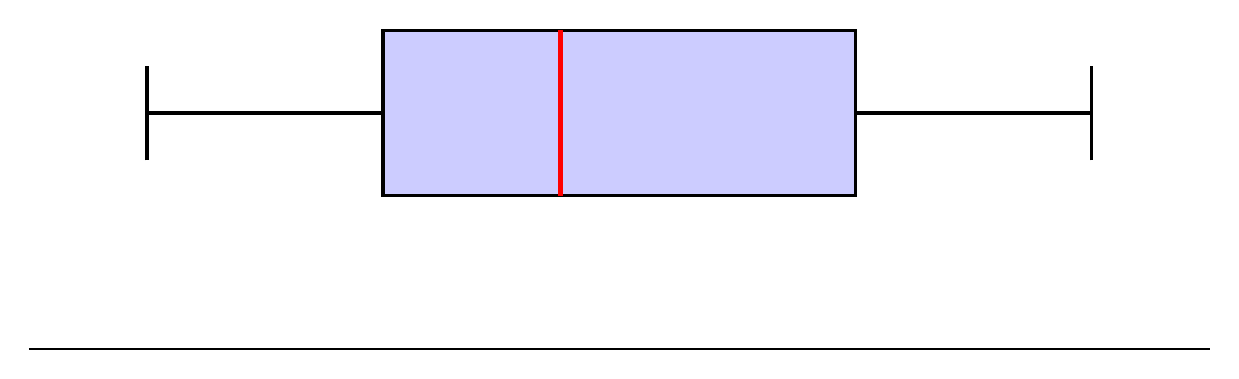
\begin{tikzpicture}[scale=1.5]
        % 横軸
        \draw[thick] (0, 0) -- (10, 0);

        % 箱ひげ図 (y=2の位置)
        \draw[very thick] (1, 2) -- (9, 2); % ひげ(最小値〜最大値)
        \draw[very thick] (1, 1.6) -- (1, 2.4); % 最小値の線
        \draw[very thick] (9, 1.6) -- (9, 2.4); % 最大値の線
        \fill[blue!20] (3, 1.3) rectangle (7, 2.7); % 箱(Q1〜Q3)
        \draw[very thick] (3, 1.3) rectangle (7, 2.7); % 箱の枠線
        \draw[very thick, red, line width=2pt] (4.5, 1.3) -- (4.5, 2.7); % 中央値

    \end{tikzpicture}
    \caption{}
    \label{fig:boxplot}
\end{figure}

% 箱ひげ図
\begin{definitionbox}[def:箱ひげ図]{\textbf{箱ひげ図}}
    図\ref{fig:boxplot}を \textbf{箱ひげ図} という。
    箱ひげ図は、データの最小値、第1四分位数、中央値(第2四分位数)、第3四分位数、最大値を箱とひげで表している。
    箱の横の長さは、四分位範囲を表す。
\end{definitionbox}

\newpage
